% gc-16-3d.tex

\documentclass[xcolor=dvipsnames]{beamer}
\usepackage{teachbeamer}

\title{Multivariable Calculus}
\subtitle{{\CourseNumber}, BCIT}

\author{\CourseName}

\date{May 8, 2018}

\begin{document}

\begin{frame}
  \titlepage
\end{frame}

\begin{frame}
  \frametitle{Function of Multiple Variables}
  Let $A$ be a domain and $B$ a codomain (both of these objects are
  sets). Then $f$ is a function from $A$ to $B$ if and only if for
  each $a\in{}A$ there is a $b\in{}B$ such that
  \begin{equation}
    \label{eq:saetohbo}
    (a,b)\in{}f
  \end{equation}
where $f$ is a set of ordered pairs consisting of pairs with an
element of $A$ in the first position and an element of $B$ in the
second position. This is the set theory of functions. Usually, we
think of $f$ as a rule which assigns to each element of $A$ an element
of $B$.
\begin{equation}
  \label{eq:oghaphah}
  f(a)=b
\end{equation}
\end{frame}

\begin{frame}
  \frametitle{Functions with Multiple Arguments}
  We can use this definition for functions with multiple
  arguments. For example, let $A$ be a subset of the $xy$ plane (the
  domain) and $B$ be a set of real numbers $z$. Then $f$ is a function
  from $A$ to $B$ if and only if for each element of $A$ there is a
  unique element of $B$ which is assigned to it.
  \begin{equation}
    \label{eq:shahthei}
    f(x,y)=z
  \end{equation}
\end{frame}

\begin{frame}[fragile]
  \frametitle{Graphical Representations: 3D}
  Here is some octave (matlab) code that simulates three dimensions in
  the plane using colours.
\begin{alltt}
x=linspace(-2,2,50);\newline
y=linspace(-2,2,50);\newline
[xx,yy]=meshgrid(x,y);\newline
mesh(xx,yy,4-(xx.^2+yy.^2))
\end{alltt}
\end{frame}

\begin{frame}
  \frametitle{Graphical Representations: 3D}
  \begin{figure}[h]
    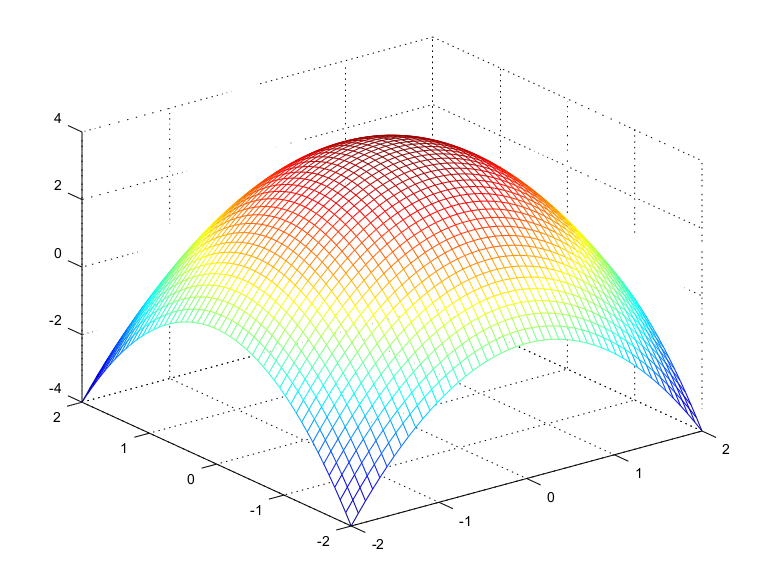
\includegraphics[scale=0.5]{./diagrams/octave-01.png}
  \end{figure}
\end{frame}

\begin{frame}
  \frametitle{Graphical Representations: Cross-Sections}
  \begin{figure}[h]
    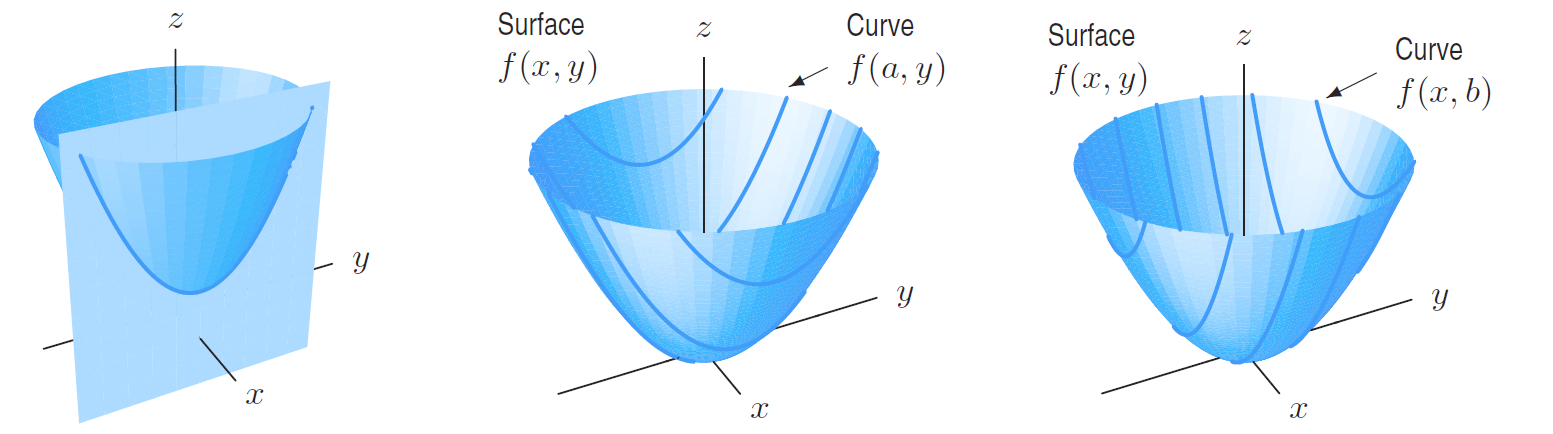
\includegraphics[scale=0.35]{./diagrams/hallett-01.png}
  \end{figure}
\end{frame}

\begin{frame}
  \frametitle{Graphical Representations: Contour Lines}
  \begin{figure}[h]
    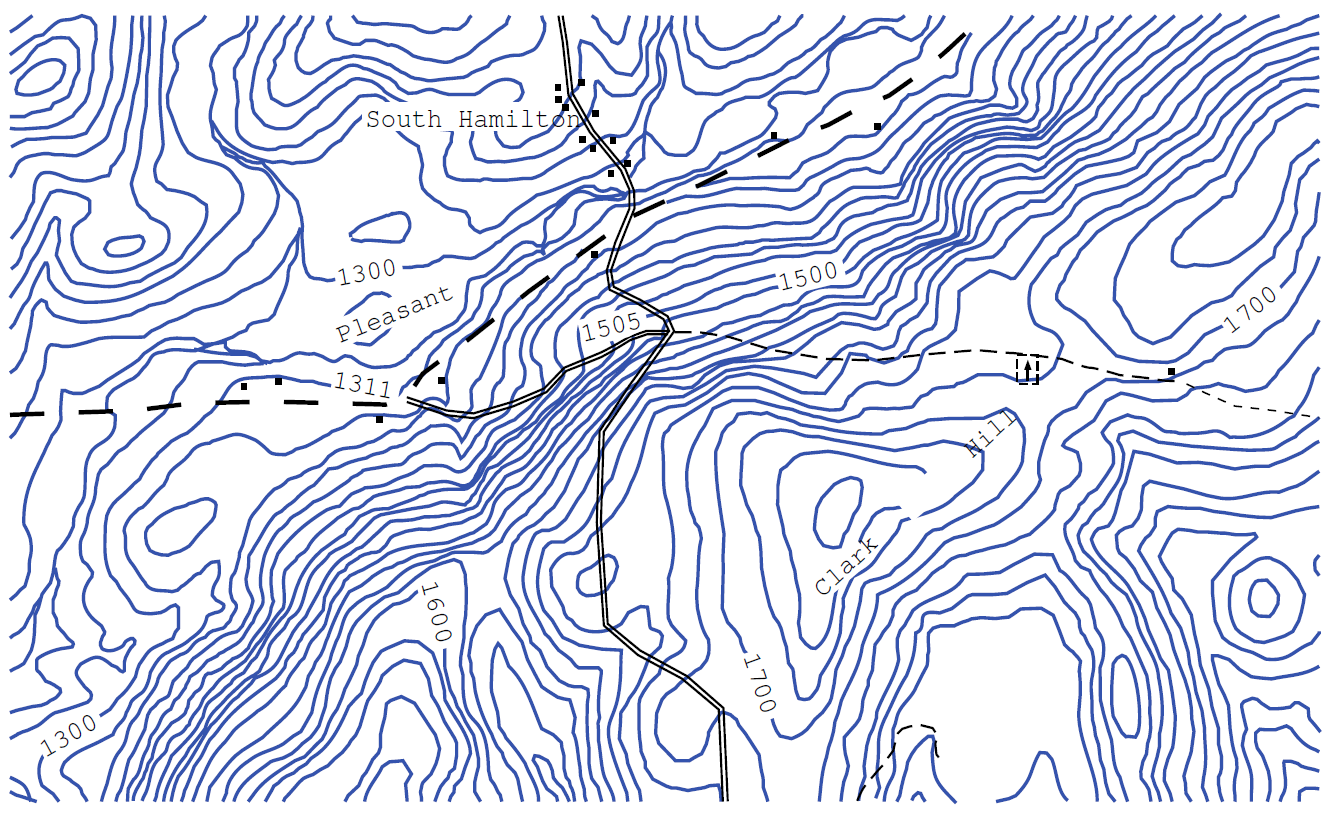
\includegraphics[scale=0.4]{./diagrams/hallett-02.png}
  \end{figure}
\end{frame}

\begin{frame}
  \frametitle{Linear Functions}
  A linear function in three-dimensional space is characterized by
  three one-dimensional parameters, just as a linear function in
  two-dimensional space is characterized by two one-dimensional
  parameters (slope and $y$-intercept). There are many different ways,
  however, to conceive of these parameters. They may be three points
  that are not all on the same line; or a point and two slopes. We
  shall define a plane or a linear function in three-dimensional space
  to be the function
  \begin{equation}
    \label{eq:oohuthah}
    f(x,y)=z_{0}+m(x-x_{0})+n(y-y_{0})
  \end{equation}
where $P=(x_{0},y_{0},z_{0})$ is a point on the plane and $m$ and $n$
are the respective slopes along the $x$-axis and the $y$-axis.
\end{frame}

\begin{frame}
  \frametitle{Linear Function Exercise}
  {\ubung} Find the linear function $f(x,y)=z$ for which the following three points are on
  the graph:
  \begin{equation}
    \label{eq:oareequu}
    \begin{array}{rcl}
      P_{1}&=&(1,0,1) \\
      P_{2}&=&(1,-1,3) \\
      P_{3}&=&(3,0,-1)
    \end{array}
  \end{equation}
\end{frame}

\begin{frame}
  \frametitle{Vectors}
  A vector is an ordered pair or triplet of real numbers. One way to interpret it
  is to make it refer to a point in the $xy$-plane or
  $xyz$-three-dimensional space. The usual interpretation, however, is
  as a \alert{displacement vector} with a direction and a length. Here
  is an example:
  \begin{equation}
    \label{eq:lapheeka}
    \vec{v}=\left(
    \begin{array}{c}
      3 \\
      5 \\
      -1
    \end{array}\right)
  \end{equation}
\end{frame}

\begin{frame}
  \frametitle{Vector Algebra}
  Vectors can be added, subtracted, and multiplied by a scalar (a real
  number).
  \begin{equation}
    \label{eq:kaepuema}
    \left(
    \begin{array}{c}
      3 \\
      5 \\
      -1
    \end{array}\right)+
  \left(
    \begin{array}{c}
      2 \\
      \pi \\
      -6
    \end{array}\right)=
  \left(
    \begin{array}{c}
      5 \\
      5+\pi \\
      -7
    \end{array}\right)
  \end{equation}
  \begin{equation}
    \label{eq:kemodaim}
    1.5\cdot\left(
    \begin{array}{c}
      3 \\
      5 \\
      -1
    \end{array}\right)=
  \left(
    \begin{array}{c}
      4.5 \\
      7.5 \\
      -1.5
    \end{array}\right)
  \end{equation}
\end{frame}

\begin{frame}
  \frametitle{Unit Vectors}
  All three-dimensional vectors can be expressed in components. For
  this expression we need unit vectors. Any three linearly-independent
  vectors would work, but it makes sense to use the following three:
  \begin{equation}
    \label{eq:bahniech}
    \vec{i}=\left(
    \begin{array}{c}
      1 \\
      0 \\
      0
    \end{array}\right)\hspace{.2in}
    \vec{j}=\left(
    \begin{array}{c}
      0 \\
      1 \\
      0
    \end{array}\right)\hspace{.2in}
    \vec{k}=\left(
    \begin{array}{c}
      0 \\
      0 \\
      1
    \end{array}\right)
  \end{equation}
\end{frame}

\begin{frame}
  \frametitle{Vector Decomposition}
  For any vector $\vec{v}$  (assuming from now on three dimensions),
  \begin{equation}
    \label{eq:teequahg}
    \vec{v}=v_{x}\vec{i}+v_{y}\vec{j}+v_{z}\vec{k}
  \end{equation}
where $V=(v_{x},v_{y},v_{z})$, and $V$ is the point to which the
origin $O=(0,0,0)$ would be displaced by vector
\begin{equation}
  \label{eq:zaegiexo}
  \vec{v}=\left(
    \begin{array}{c}
      v_{x} \\
      v_{y} \\
      v_{z} \\
    \end{array}\right)
\end{equation}
\end{frame}

\begin{frame}
  \frametitle{Vector Length and Distance Between Two Points}
  The length of vector $\vec{v}$ is
  \begin{equation}
    \label{eq:ogeithie}
    \Vert\vec{v}\Vert=\sqrt{v_{x}^{2}+v_{y}^{2}+v_{z}^{2}}
  \end{equation}
The distance between two points $P$ and $Q$ is the length of a
displacement vector between them. Let $\vec{OP}$ be the displacement
vector from $O$ to $P$ and so on. Then
\begin{equation}
  \label{eq:ahnoocae}
  \vec{PQ}=\vec{PO}+\vec{OQ}=\vec{OQ}-\vec{OP}
\end{equation}
and $\Vert\vec{PQ}\Vert$ is the distance between $P$ and $Q$.
\end{frame}

\begin{frame}
  \frametitle{Dot Product}
  The following two definition of the \alert{dot product}, or
  \alert{scalar product}, $\vec{v}\cdot\vec{w}$ are equivalent:
  \begin{description}
  \item[geometric]
    $\vec{v}\cdot\vec{w}=\Vert\vec{v}\Vert\cdot\Vert\vec{w}\Vert\cdot\cos\vartheta$
    where $\vartheta$ is the angle between $\vec{v}$ and $\vec{w}$,
    $0\leq\vartheta\leq\pi$.
  \item[algebraic] $\vec{v}\cdot\vec{w}=v_{x}w_{x}+v_{y}w_{y}+v_{z}w_{z}$
  \end{description}
The dot product is a number, not a vector.
\end{frame}

\begin{frame}
  \frametitle{Dot Product}
  Now we need to show that the two definitions are equivalent.
  Consider a triangle $PQR$ in three-dimensional space. Let
  $\vec{v}=\vec{PQ},\vec{w}=\vec{PR}$. Then
  \begin{equation}
    \label{eq:oobeipho}
  \vec{QR}=\vec{QP}+\vec{PR}=-\vec{v}+\vec{w}=\vec{w}-\vec{v}  
\end{equation}
Here is the law of cosines for this triangle:
\begin{equation}
  \label{eq:aiwahzoa}
  \Vert\vec{w}-\vec{v}\Vert^{2}=\Vert\vec{v}\Vert^{2}+\Vert\vec{w}\Vert^{2}-2\Vert\vec{v}\Vert\cdot\Vert\vec{w}\Vert\cos\vartheta
\end{equation}
It follows that the two definitions are equivalent.
\end{frame}

\begin{frame}
  \frametitle{Dot Product}
\begin{block}{Perpendicularity and Dot Product}
  Two non-zero vectors $\vec{v}$ and $\vec{w}$ are perpendicular, or
  orthogonal, if and only if $\vec{v}\cdot\vec{w}=0$.
\end{block}

\bigskip

\begin{block}{Magnitude and Dot Product}
  Magnitude and dot product are related as follows: $\vec{v}\cdot\vec{v}=\Vert\vec{v}\Vert$.
\end{block}
\end{frame}

% this is NOT correct
% \begin{frame}
%   \frametitle{Dot Product Exercise}
%   {\ubung} Find a normal vector to the following planes (a normal vector to a
%   plane is perpendicular to all non-zero vectors displacing points on
%   the plane).
%   \begin{equation}
%     \label{eq:afanaagu}
%     2x+y-z=5
%   \end{equation}
%   \begin{equation}
%     \label{eq:reeregha}
%     2(x-z)=3(x+y)
%   \end{equation}
%   For (\ref{eq:afanaagu}), set $x=1,y=1$, then $z=-2$ for
%   $P=(1,1,-2)$. Then set $x=3,y=1$, so $z=2$ for $Q=(3,1,2)$. Both $P$
%   and $Q$ are on the plane, so $\vec{PQ}=\vec{OQ}-\vec{OP}$ is a
%   vector displacing two points in the plane. To find a vector
%   perpendicular to it consider the dot product
% \begin{equation}
%   \label{eq:chiemaig}
%   -2x+0y-4z=0
% \end{equation}
% Choose $x=1,y=1$, so $z=-0.5$. The vector
% $1\cdot\vec{i}+1\cdot\vec{j}-0.5\cdot\vec{k}$ is a normal vector to the
% plane $2x+y-z=5$.
% \end{frame}

\begin{frame}
  \frametitle{Dot Product Exercise}
  {\ubung} Find the angle between
  \begin{equation}
    \label{eq:tauhohju}
    \vec{v}=\left(
      \begin{array}{c}
        4 \\
        0 \\
        7
      \end{array}\right)\hspace{.5in}\vec{w}=\left(
      \begin{array}{c}
        -2 \\
        1 \\
        3
      \end{array}\right)
  \end{equation}
  Consider the dot product
  \begin{equation}
    \label{eq:ijaquahd}
    4\cdot(-2)+0\cdot{}1+7\cdot{}3=13
  \end{equation}
According to the two equivalent definitions of the dot product, this
is equal to
\begin{equation}
  \label{eq:ohyizaeb}
  \Vert\vec{v}\Vert\cdot\Vert\vec{w}\Vert\cdot\cos\vartheta=\sqrt{4^{2}+7^{2}}\cdot\sqrt{(-2)^{2}+1^{2}+3^{2}}\cdot\cos\vartheta
\end{equation}
Therefore,
\begin{equation}
  \label{eq:yohsheen}
  \vartheta=\arccos\frac{13}{\sqrt{4^{2}+7^{2}}\cdot\sqrt{(-2)^{2}+1^{2}+3^{2}}}=64.47^{\circ}
\end{equation}
\end{frame}

\begin{frame}
  \frametitle{Planes Again}
  The equation of the plane with normal vector
  $\vec{n}=a\vec{i}+b\vec{j}+c\vec{k}$ and containing the point
  $P=(x_{0},y_{0},z_{0})$ is
  \begin{equation}
    \label{eq:ijaeriri}
    a(x-x_{0})+b(y-y_{0})+c(z-z_{0})=0
  \end{equation}
  Alternatively, for $d=ax_{0}+by_{0}+cz_{0}$
  \begin{equation}
    \label{eq:bamoyeez}
    ax+by+cz=d
  \end{equation}
\end{frame}

\begin{frame}
  \frametitle{Cross Product}
  \begin{figure}[h]
    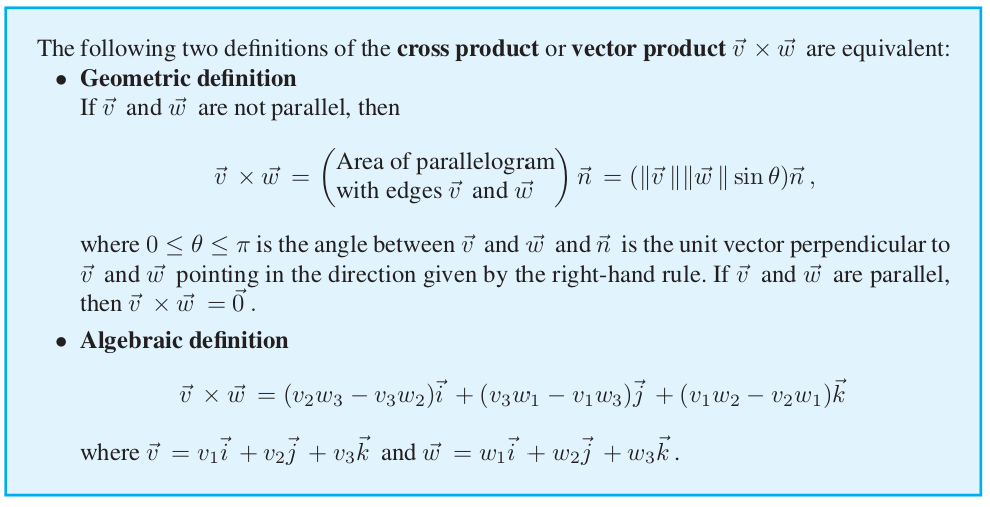
\includegraphics[scale=0.32]{./diagrams/crossproduct.png}
  \end{figure}
\end{frame}

\begin{frame}
  \frametitle{Cross Product}
  If you know what a determinant is, you can remember the algebraic
  definition as follows.
  \begin{equation}
    \label{eq:abeekohc}
    \vec{v}\times\vec{w}=\left\vert
      \begin{array}{ccc}
        \vec{i} & \vec{j} & \vec{k} \\
        v_{1} & v_{2} & v_{3} \\
        w_{1} & w_{2} & w_{3}
      \end{array}\right\vert
  \end{equation}
  Note that $\vec{w}\times\vec{v}=-\vec{v}\times\vec{w}$.
\end{frame}

\begin{frame}
  \frametitle{Cross Product Exercise}
  {\ubung} Use the cross product to find the linear equation containing the
  three points
  \begin{equation}
    \label{eq:eiyeigaz}
    \begin{array}{rcl}
      P&=&(1,3,0) \\
      Q&=&(3,4,-3) \\
      R&=&(3,6,2)
    \end{array}
  \end{equation}
\end{frame}

\begin{frame}
  \frametitle{Cross Product Exercise Answer}
One way to find the answer to the last exercise (without using the
cross product) is to solve the following system of linear equations
for the plane $x+ay+bz=c$,
\begin{equation}
  \label{eq:yohghaef}
  \begin{array}{rcl}
    1+3a+0b&=&c \\
    3+4a-3b&=&c \\
    3+6a+2b&=&c
  \end{array}
\end{equation}
Change this to
\begin{equation}
  \label{eq:oxeingiu}
  \begin{array}{rcl}
    3a+0b-c&=&-1 \\
    4a-3b-c&=&-3 \\
    6a+2b-c&=&-3 \\
  \end{array}
\end{equation}
Using matrices,
\begin{equation}
  \label{eq:ukohjiej}
  \left(
    \begin{array}{ccc}
      3&0&-1 \\
      4&-3&-1 \\
      6&2&-1
    \end{array}\right)\cdot\left(
    \begin{array}{c}
      a \\
      b \\
      c
    \end{array}\right)=\left(
    \begin{array}{c}
      -1 \\
      -3 \\
      -3
    \end{array}\right)
\end{equation}
\end{frame}

\begin{frame}
  \frametitle{Cross Product Exercise Answer}
  Equation (\ref{eq:ukohjiej}) yields the solution
  \begin{equation}
    \label{eq:maeshael}
      x-\frac{10}{11}y+\frac{4}{11}z=-\frac{19}{11}
  \end{equation}
Now let's use the cross product instead, avoiding the matrices. Note
that
\begin{equation}
  \label{eq:ushahroh}
  \begin{array}{rcl}
    \vec{PQ}&=&2\vec{i}+\vec{j}-3\vec{k} \\
    \vec{PR}&=&2\vec{i}+3\vec{j}+2\vec{k}
  \end{array}
\end{equation}
The cross product, using the algebraic definition, is
$\vec{u}=\vec{PQ}\times\vec{PR}=11\vec{i}-10\vec{j}+4\vec{k}$.
\end{frame}

\begin{frame}
  \frametitle{Cross Product Exercise Answer}
  Let $P=(x_{0},y_{0},z_{0})$ be a fixed point on the plane with known
  coordinates. Since any point $S=(x,y,z)$ on the plane fulfills
\begin{equation}
  \label{eq:iefeeboh}
  \vec{PS}\cdot\vec{u}=0
\end{equation}
this can be turned into the plane equation
\begin{equation}
  \label{eq:vetiexup}
  u_{x}(x-x_{0})+u_{y}(y-y_{0})+u_{z}(z-z_{0})=0
\end{equation}
Therefore, using $P=(1,3,0)$, this translates into
\begin{equation}
  \label{eq:eechawoi}
11x-10y+4z=19  
\end{equation}
which is equivalent to (\ref{eq:maeshael}). Notice how easy it is to
find a linear equation when you have a point $P=(x_{0},y_{0},z_{0})$
on the plane and a normal vector $\vec{u}$ to the plane
$u_{x}\vec{i}+u_{y}\vec{j}+u_{z}\vec{k}$:
\begin{equation}
  \label{eq:quaghoob}
u_{x}x+u_{y}y+u_{z}z=u_{x}x_{0}+u_{y}y_{0}+u_{z}z_{0}
\end{equation}
\end{frame}

\begin{frame}
  \frametitle{Partial Derivatives}
  The derivative of a one-variable function measures its rate of
  change. We will see how a two-variable function has two rates of
  change: one as $x$ changes (with $y$ held constant) and one as $y$ changes
  (with $x$ held constant).

  \bigskip

  For all points at which the limits exist, we define the
  \alert{partial derivatives} at the point $(a,b)$ by
  \begin{equation}
    \label{eq:deeghazi}
    f_{x}(a,b)=\lim_{h\rightarrow{}0}\frac{f(a+h,b)-f(a,b)}{h}
  \end{equation}
  \begin{equation}
    \label{eq:aevoonei}
    f_{y}(a,b)=\lim_{h\rightarrow{}0}\frac{f(a,b+h)-f(a,b)}{h}
  \end{equation}
If we let $a$ and $b$ vary, we have the \alert{partial derivative
  functions} $f_{x}(x,y)$ and $f_{y}(x,y)$. 
\end{frame}

\begin{frame}
  \frametitle{Partial Derivatives Notation}
  There is some terrifying notation for partial derivatives. If
  $z=f(x,y)$, we can write
  \begin{equation}
    \label{eq:eequaeru}
f_{x}(x,y)=\frac{\partial{}z}{\partial{}x}\mbox{ and }f_{y}(x,y)=\frac{\partial{}z}{\partial{}y}
  \end{equation}
  \begin{equation}
    \label{eq:quohkahr}
f_{x}(a,b)=\left.\frac{\partial{}z}{\partial{}x}\right\vert_{(a,b)}\mbox{ and }f_{y}(a,b)=\left.\frac{\partial{}z}{\partial{}y}\right\vert_{(a,b)}
  \end{equation}
\end{frame}

\begin{frame}
  \frametitle{Partial Derivatives}
  \begin{figure}[h]
    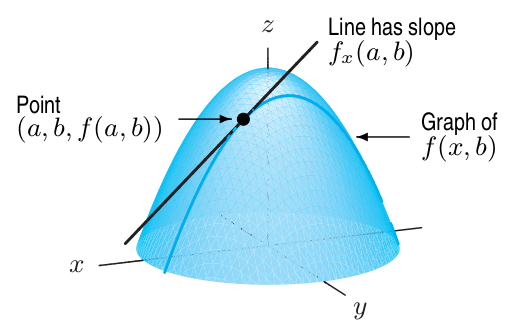
\includegraphics[scale=0.5]{./diagrams/partialx.png}
  \end{figure}
\end{frame}

\begin{frame}
  \frametitle{Partial Derivatives}
  \begin{figure}[h]
    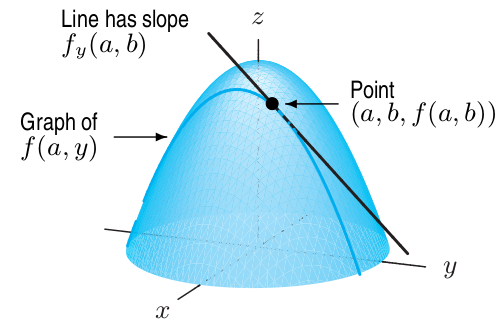
\includegraphics[scale=0.5]{./diagrams/partialy.png}
  \end{figure}
\end{frame}

\begin{frame}
  \frametitle{Tangent Planes}
  Assuming $f$ is differentiable at $(a,b)$, the equation of the
  tangent plane is
  \begin{equation}
    \label{eq:aoseenai}
z=f(a,b)+f_{x}(a,b)(x-a)+f_{y}(a,b)(y-b)
  \end{equation}
  $f(x,y)$ can be approximated around $(a,b)$ by the tangent plane,
  \begin{equation}
    \label{eq:xabixaic}
    f(x,y)\approx{}f(a,b)+f_{x}(a,b)(x-a)+f_{y}(a,b)(y-b)\mbox{ near }(a,b)
  \end{equation}
\end{frame}

\begin{frame}
  \frametitle{Partial Derivatives Exercise}
  {\ubung} Let
  \begin{equation}
    \label{eq:oacheapo}
    f(x,y)=\frac{x^{2}}{y+1}
  \end{equation}
  Find $f_{x}(3,2)$.

  \bigskip

  {\ubung} Compute the partial derivatives with respect to $x$ and
  with respect to $y$ for the following functions.
  \begin{equation}
    \label{eq:phiwoowe}
    f(x,y)=y^{2}e^{3x}
  \end{equation}
  \begin{equation}
    \label{eq:uphaijei}
    z=(3xy+2x)^{5}
  \end{equation}
  \begin{equation}
    \label{eq:geebeshi}
    g(x,y)=e^{x+3y}\sin(xy)
  \end{equation}
\end{frame}

\begin{frame}
  \frametitle{Second Order Partial Derivatives}
  The \alert{second order partial derivatives} are
  \begin{equation}
    \label{eq:eshaipie}
    \frac{\partial^{2}z}{\partial{}x^{2}}=f_{xx}=\left(f_{x}\right)_{x}\hspace{0.5in}\frac{\partial^{2}z}{\partial{}x\partial{}y}=f_{yx}=\left(f_{y}\right)_{x}
  \end{equation}
  \begin{equation}
    \label{eq:waukahna}
    \frac{\partial^{2}z}{\partial{}y\partial{}x}=f_{xy}=\left(f_{x}\right)_{y}\hspace{0.5in}\frac{\partial^{2}z}{\partial{}y^{2}}=f_{yy}=\left(f_{y}\right)_{y}
  \end{equation}
  It turns out that if $f_{xy}$ and $f_{yx}$ are continuous at
  $(a,b)$, then
  \begin{equation}
    \label{eq:ahbahxuj}
    f_{xy}(a,b)=f_{yx}(a,b)
  \end{equation}
\end{frame}

\begin{frame}
  \frametitle{Saddle Points}
  consider the following function graph:
  \begin{figure}[h]
    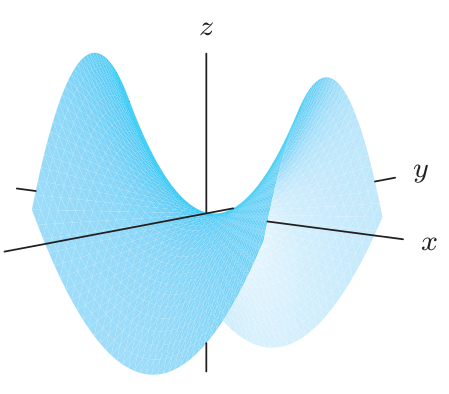
\includegraphics[scale=0.35]{./diagrams/saddle.png}
  \end{figure}
  Is $f_{xx}(0,0)$ positive or negative? Is $f_{yy}(0,0)$ positive or negative? 
\end{frame}

\begin{frame}
  \frametitle{Critical Points}
  $f$ has a \alert{local maximum} at the point $P_{0}$ if $f(P_{0})\geq{}f(P)$
  for all points $P$ near $P_{0}$.

  \bigskip

  $f$ has a \alert{local minimum} at the point $P_{0}$ if $f(P_{0})\leq{}f(P)$
  for all points $P$ near $P_{0}$.
\end{frame}

\begin{frame}
  \frametitle{Critical Points}
  \begin{figure}[h]
    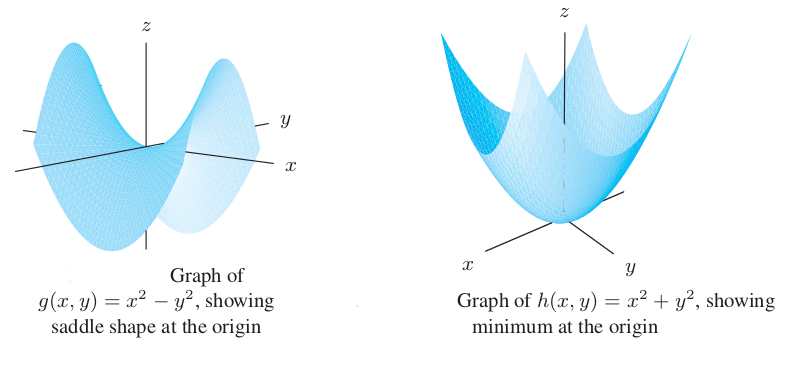
\includegraphics[scale=0.42]{./diagrams/critpoints.png}
  \end{figure}
\end{frame}

\begin{frame}
  \frametitle{Second-Derivative Test for Functions of Two Variables}
  Suppose $(x_{0},y_{0})$ is a point where the partial derivatives are
  both 0. Let
  \begin{equation}
    \label{eq:eezongoo}
    D=f_{xx}(x_{0},y_{0})f_{yy}(x_{0},y_{0})-(f_{xy}(x_{0},y_{0}))^{2}
  \end{equation}
  Then
  \begin{itemize}
  \item If $D>0$ and $f_{xx}(x_{0},y_{0})>0$, then $f$ has a local minimum at $(x_{0},y_{0})$.
  \item If $D>0$ and $f_{xx}(x_{0},y_{0})<0$, then $f$ has a local maximum at $(x_{0},y_{0})$.
  \item If $D<0$, then $f$ has a saddle point at $(x_{0},y_{0})$.
  \item If $D=0$, then anything can happen: $f$ can have a local maximum, or a local minimum, or a saddle point, or none of these, at $(x_{0},y_{0})$.
  \end{itemize}
\end{frame}

\begin{frame}
  \frametitle{Optimization Exercise}
  {\ubung} Find the local maxima, minima, and saddle points of
  \begin{equation}
    \label{eq:onahsood}
    f(x,y)=x^{2}+2y^{2}-x
  \end{equation}
  \begin{equation}
    \label{eq:enaepain}
    g(x,y)=\frac{1}{2}x^{2}+3y^{3}+9y^{2}-3xy+9y-9x
  \end{equation}
  \begin{equation}
    \label{eq:phedohde}
    h(x,y)=e^{-x^{2}-y^{2}}
  \end{equation}
\end{frame}

\begin{frame}
  \frametitle{Optimization Visual}
  \begin{figure}[h]
    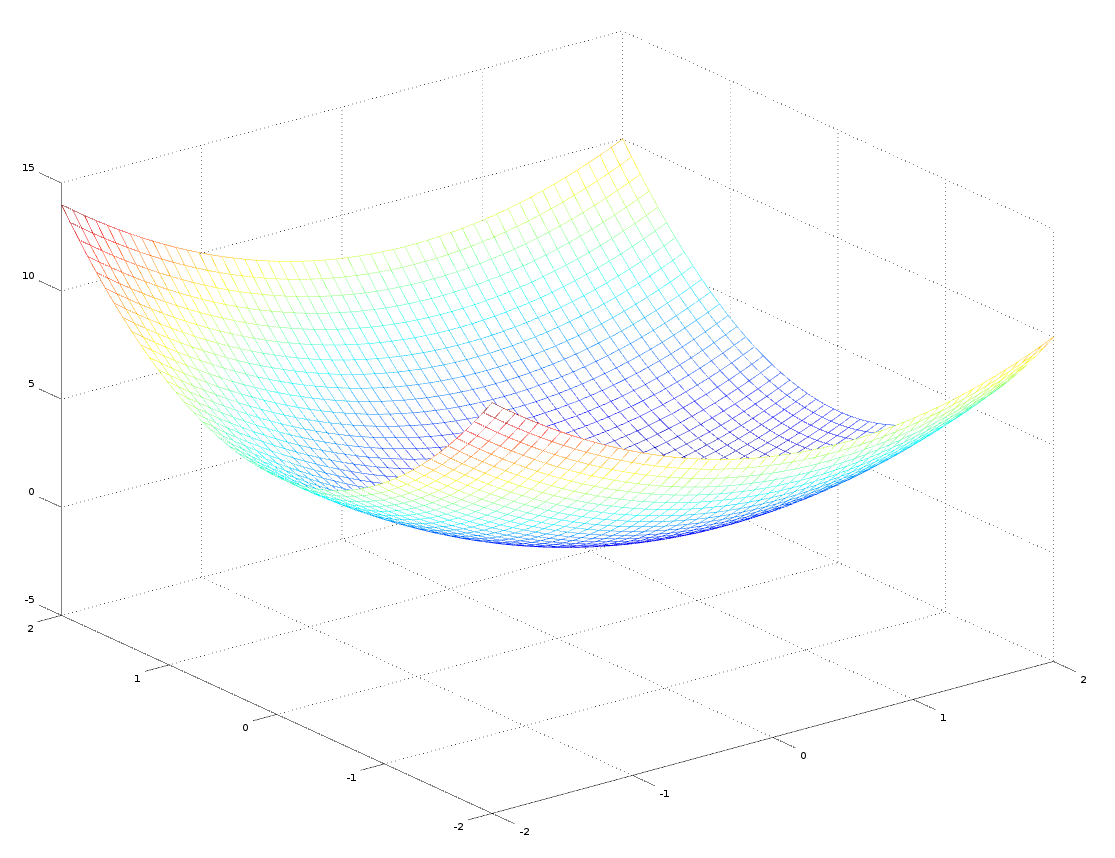
\includegraphics[scale=0.27]{./diagrams/threed1.png}
  \end{figure}
\end{frame}

\begin{frame}
  \frametitle{Optimization Visual}
  \begin{figure}[h]
    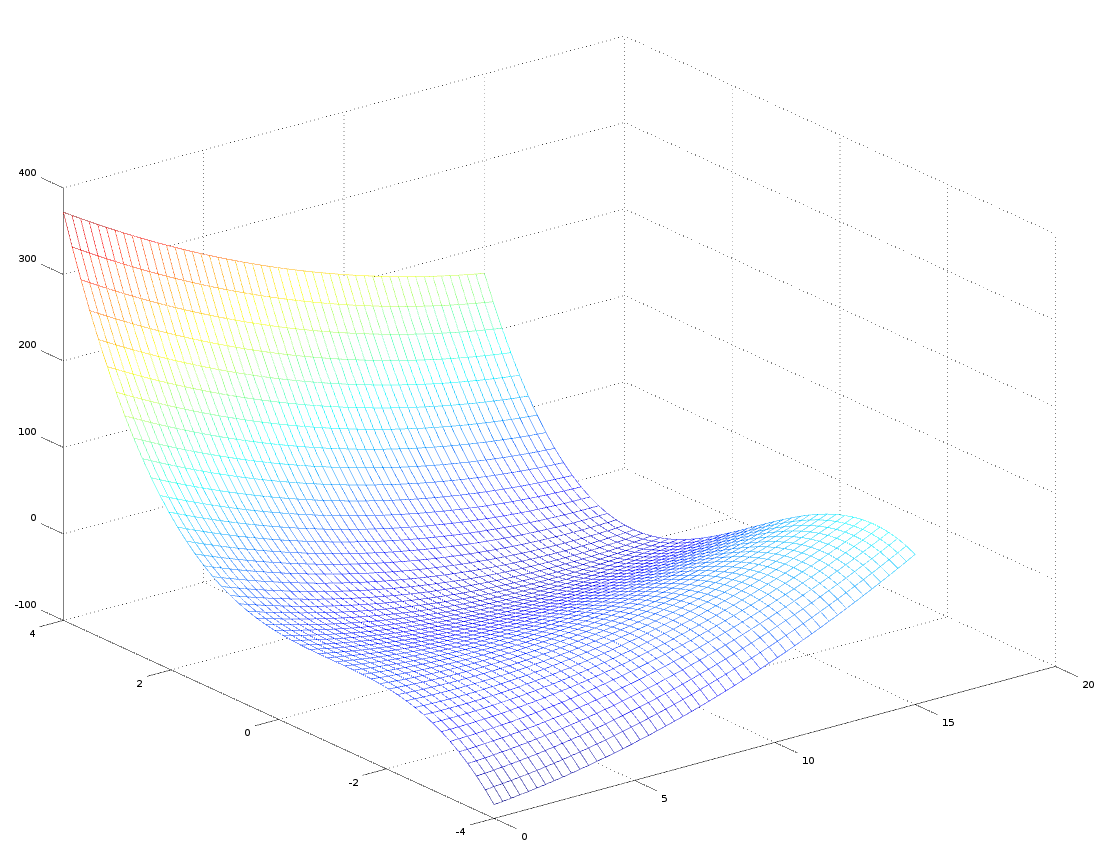
\includegraphics[scale=0.27]{./diagrams/threed2.png}
  \end{figure}
\end{frame}

\begin{frame}
  \frametitle{Optimization Visual}
  \begin{figure}[h]
    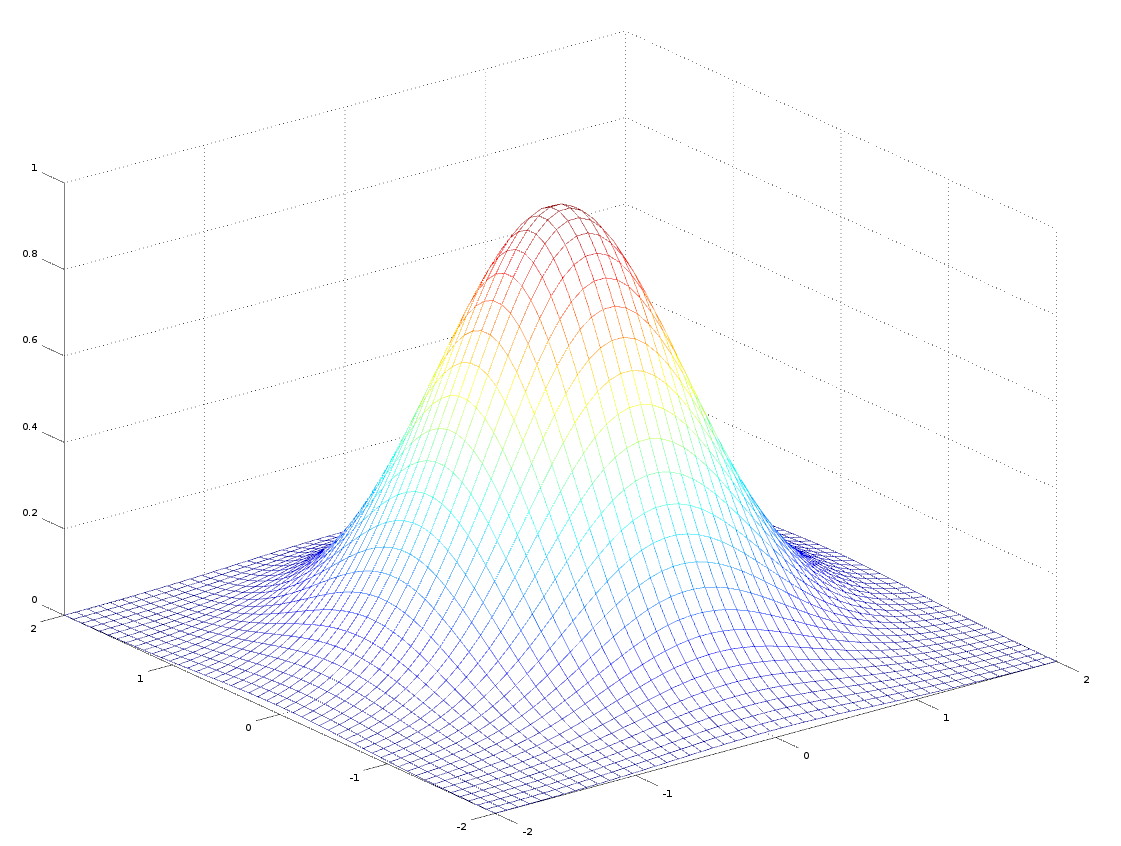
\includegraphics[scale=0.27]{./diagrams/threed3.png}
  \end{figure}
\end{frame}

\begin{frame}
  \frametitle{Optimization Exercise}
  {\ubung} A delivery of 480 cubic meters of gravel is to be made
  to a landfill. The trucker plans to purchase an open-top box in
  which to transport the gravel in numerous trips. The total cost
  to the trucker is the cost of the box plus \$80 per trip. The
  box must have height 2 metres, but the trucker can choose the
  length and width. The cost of the box is \$100/$m^{2}$ for the
  ends, \$50/$m^{2}$ for the sides and \$200/$m^{2}$ for the
  bottom. Notice the tradeoff: A smaller box is cheaper to buy but
  requires more trips. What size box should the trucker buy to
  minimize the total cost?
\end{frame}

\begin{frame}
  \frametitle{Judy Benjamin}
  \begin{figure}[h]
    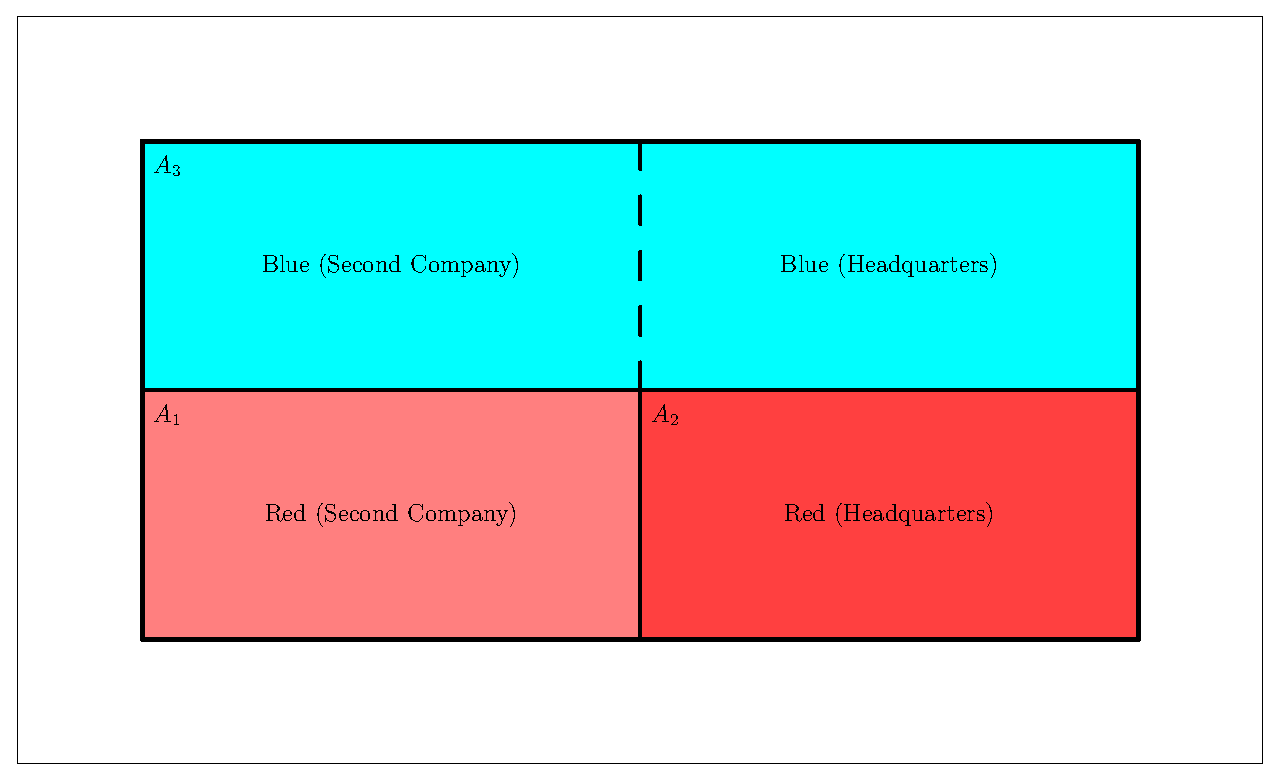
\includegraphics[scale=0.5]{./diagrams/judy.eps}
  \end{figure}
\end{frame}

\begin{frame}
  \frametitle{Judy Benjamin}
\begin{itemize}
\item (MAP) Judy has no idea where she is. She is on team Blue.
  Because of the map, her probability of being in Blue territory
  equals the probability of being in Red territory, and being on Red
  Second Company ground equals the probability of being on Red
  Headquarters ground.
\item (HDQ) Headquarters inform Judy that in case she is in Red
  territory, her chance of being on their Headquarters ground is three
  times the chance of being on their Second Company ground.
\end{itemize}
\begin{equation}
  \label{eq:map}
  2\cdot{}p_{1}=2\cdot{}p_{2}=p_{3}\tag{\mbox{MAP}}
\end{equation}
\begin{equation}
  \label{eq:hdq}
  \frac{q_{2}}{q_{3}}=3\tag{\mbox{HDQ}}
\end{equation}
\end{frame}

\begin{frame}
  \frametitle{The Principle of Maximum Entropy}
\begin{figure}[h]
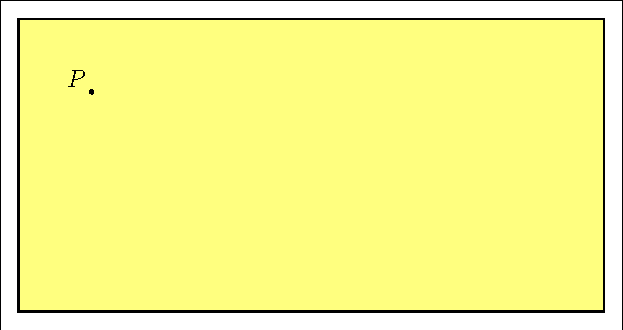
\includegraphics[scale=1.0]{constraint-a.pdf}
\end{figure}
\end{frame}

\begin{frame}
  \frametitle{The Principle of Maximum Entropy}
\begin{figure}[h]
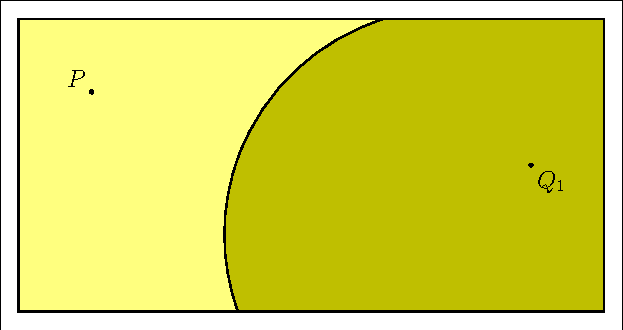
\includegraphics[scale=1.0]{constraint-b.pdf}
\end{figure}
\end{frame}

\begin{frame}
  \frametitle{The Principle of Maximum Entropy}
\begin{figure}[h]
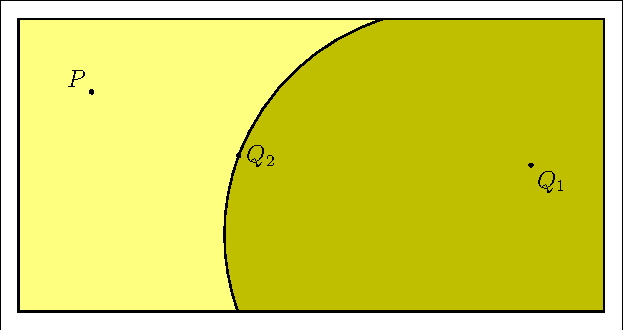
\includegraphics[scale=1.0]{constraint-c.pdf}
\end{figure}
\end{frame}

\begin{frame}
  \frametitle{The Principle of Maximum Entropy}
\begin{figure}[h]
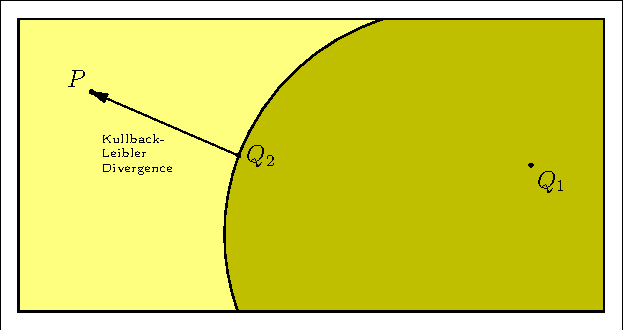
\includegraphics[scale=1.0]{constraint-d.pdf}
\end{figure}
\end{frame}

\begin{frame}
  \frametitle{Kullback-Leibler Divergence}
  The Kullback-Leibler Divergence is
\begin{equation}
  \label{eq:kl}
  D(Q,P)=\sum_{i=1}^{m}q_{i}\log_{2}\frac{q_{i}}{p_{i}}\notag
\end{equation}
Our point $P=(0.5,0.25,0.25)$ is fixed. Define the function
\begin{equation}
  \label{eq:nughaoqu}
  f(q_{1},q_{2},q_{3})=q_{1}\log\frac{q_{1}}{0.5}+q_{2}\log\frac{q_{2}}{0.25}+q_{3}\log\frac{q_{3}}{0.25}
\end{equation}
and find the minimum with the constraint that $q_{1}+q_{2}+q_{3}=1$
and $q_{2}=3q_{3}$.
\end{frame}

\begin{frame}
  \frametitle{Lagrange Multipliers}
  The function with Lagrange Multipliers is
  \begin{equation}
    \label{eq:eoreaque}
    LM(q_{1},q_{2},q_{3},\lambda,\mu)=q_{1}\log\frac{q_{1}}{0.5}+q_{2}\log\frac{q_{2}}{0.25}+q_{3}\log\frac{q_{3}}{0.25}+\notag
  \end{equation}
  \begin{equation}
    \label{eq:okeexeim}
    \lambda(q_{1}+q_{2}+q_{3}-1)+\mu(q_{2}-3q_{3})
  \end{equation}
Differentiation with respect to $\lambda$ and $\mu$ and setting to
zero gives you the two constraints.
\begin{equation}
  \label{eq:iceekasu}
  \frac{\partial{}LM}{\partial{}q_{1}}=\log\frac{q_{1}}{0.5}+1+\lambda
\end{equation}
\begin{equation}
  \label{eq:theiquae}
  \frac{\partial{}LM}{\partial{}q_{2}}=\log\frac{q_{2}}{0.25}+1+\lambda+\mu
\end{equation}
\begin{equation}
  \label{eq:laxiexeo}
  \frac{\partial{}LM}{\partial{}q_{3}}=\log\frac{q_{3}}{0.25}+1+\lambda-3\mu
\end{equation}
\end{frame}

\begin{frame}
  \frametitle{Lagrange Multipliers}
  Setting (\ref{eq:iceekasu})--(\ref{eq:laxiexeo}) to zero with these
  two constraints gives us a system of five equations with five
  variables.
  \begin{equation}
    \label{eq:gooxique}
    q_{1}=\frac{1}{2}e^{1+\lambda}
  \end{equation}
  \begin{equation}
    \label{eq:aedeenoh}
    q_{2}=\frac{1}{4}e^{1+\lambda+\mu}
  \end{equation}
  \begin{equation}
    \label{eq:uithahju}
    q_{3}=\frac{1}{4}e^{1+\lambda-3\mu}
  \end{equation}
  \begin{equation}
    \label{eq:meeshoch}
\frac{1}{2}e^{1+\lambda}+\frac{1}{4}e^{1+\lambda+\mu}+\frac{1}{4}e^{1+\lambda-3\mu}=1
  \end{equation}
  \begin{equation}
    \label{eq:dohjohsa}
    \frac{1}{4}e^{1+\lambda+\mu}=\frac{3}{4}e^{1+\lambda-3\mu}
  \end{equation}
\end{frame}

\begin{frame}
  \frametitle{Lagrange Multipliers}
  Equation (\ref{eq:dohjohsa}) gives us $\mu=\frac{1}{4}\ln{}3$. Substituting
  this in (\ref{eq:meeshoch}) gives us
  \begin{equation}
    \label{eq:chuquohv}
    \lambda=\ln\frac{4}{e\left(2+3^{\frac{1}{4}}+3^{-\frac{3}{4}}\right)}
  \end{equation}
Substituting these values in (\ref{eq:gooxique}), (\ref{eq:aedeenoh}),
and (\ref{eq:uithahju}) yields
\begin{equation}
  \label{eq:aibigoib}
  \left(
    \begin{array}{c}
      q_{1} \\
      q_{2} \\
      q_{3}
    \end{array}\right)\approx\left(
    \begin{array}{c}
      0.533 \\
      0.350 \\
      0.117
    \end{array}\right)
\end{equation}
Surprisingly, even though the radio call from headquarters was all
about the enemy territory, Judy ought to increase her degree of belief
that she has landed in friendly territory from $0.50$ to $0.533$.
\end{frame}

\begin{frame}
  \frametitle{End of Lesson}
Next Lesson: End of Term! Have a Happy Holiday!
\end{frame}

\end{document}

